% =====================================================================
%  Section 7 -- Simulation study (owner: phase-2 SIM writer).
%  Every number is taken from results/sim_results.json (code/run_experiments.py);
%  results/SUMMARY.md prints the same values. Details in appendix/C-simulation-details.tex.
% =====================================================================
\providecommand{\Se}{\mathrm{Se}}
\providecommand{\Sp}{\mathrm{Sp}}
% Scale a table down (never up) to the line width.
\providecommand{\simfit}[1]{\resizebox{\ifdim\width>\linewidth\linewidth\else\width\fi}{!}{#1}}

\section{Simulation study}\label{sec:simulation}

This section tests the tools of \cref{sec:estimands,sec:markov,sec:identification,sec:measurement} on a synthetic recommender whose amplification is known. Every number comes from \texttt{results/sim\_results.json}, which the code in \texttt{code/} produces. No real platform, item or user is involved, and nothing here is a finding about any service. E1 evaluates the correction for misclassification (\cref{thm:misclass}), and E1b the variance estimators of \cref{thm:identify}. E2 evaluates interference (\cref{prop:interference}), E3 the decomposition of \cref{thm:decomp}, E4 the Markov model (\cref{prop:markov,thm:perturb}) and E5 the sequential audit (\cref{alg:sequential,prop:power}). \Cref{app:simdetails} gives the configurations, seeds, versions, runtimes, reproduction commands and further results. It also explains why E5 was run again after \cref{alg:sequential} was revised.

\subsection{The synthetic world}\label{sec:sim-world}

\paragraph{Catalogue and policies} The catalogue has $5{,}000$ items in six topics, embedded in eight dimensions, one of which is a direction on which antisemitic items load. Items are neutral ($4{,}401$), borderline ($399$), coded antisemitic ($100$) or explicit antisemitic ($100$), with $L_c=1$ for the last two. By construction the antisemitic share ranges from $0.6\%$ of items in sport and entertainment to $11.5\%$ in the conspiracy topic. Borderline and antisemitic items also have a higher engagement prior (``bait''), popularity and posting rate. These are assumptions, not estimates. Each slate has $k=4$ items, drawn from an eligible pool of $50$ items that is redrawn at every step from the topics that the account follows. The algorithm also considers the $15$ nearest neighbours of the current item and $15$ trending items. It ranks candidates by $2\langle v_u,x_c\rangle+0.3\log(\text{popularity}_c)+\text{bait}_c$ plus Gumbel noise, and it moves the user embedding toward each opened item, $v_u\leftarrow0.9\,v_u+0.1\,x_c$. The references of \cref{sec:est-reference} show the pool's four newest, four random, or four most popular items.

\paragraph{Classifier} An impression is flagged when a type-specific mean plus normal noise is positive. Under ND, specificity is $0.98$ on neutral and borderline items and sensitivity $0.85$ on both antisemitic types. DU flags $40\%$ of borderline items, and DD has $\Se=0.35$ on coded and $0.95$ on explicit items. NDI has the rates of ND, but its noise is fixed per item. Error never depends on the arm, so arm-level rates differ only when the arms show different mixtures of types (\cref{thm:misclass}(c)). Scores fall into five bands, of which the top two are flagged.

\paragraph{Accounts and personas} Protocol puppets (\cref{sec:prot-personas}) are trained by opening $30$ seed items from the $200$ neutral items closest to their persona. They then run $S=10$ sessions of $T=20$ steps ($800$ recorded impressions), opening at each step the highest-ranked item that is similar to the persona and scores below $\tau_{\mathrm{safe}}=-0.5$ (avoid-on-flag). The true $\mathrm{AR}(d)$ therefore depends slightly on the classifier. Naturalistic accounts (E3, E4) choose by a multinomial logit in taste, appetite for each content state, bait, position and similarity to the current item. The four personas, general interest ($d_0$), Jewish interest, Middle East news and conspiracy-adjacent, are synthetic: topic weights in the invented catalogue, with appetites for naturalistic accounts (\cref{tab:sim-config}). They describe no real group of users.

\paragraph{Interference and demand} Global popularity, which the algorithm and the popularity-only feed use, is frozen except in E2. There, puppets' openings feed it, with a half-life of one day. In E3, users' taste drifts toward what they open, and their appetite for borderline and antisemitic items rises with the share of such openings. A growing share of their pool also comes from such sources that they now follow. The Monte Carlo standard error (MCSE) of a coverage near $95\%$ is $0.7$ points with $R=1{,}000$ audits, $0.5$ with $2{,}000$, and $4.4$ with E2's $24$ replications.

\subsection{Misclassification (E1)}\label{sec:sim-misclass}

For each regime we simulated pools of $1{,}000$ protocol puppets per persona and policy, without interference. An audit draws $U\in\{5,10,20,40,80\}$ puppets per cell, $R=1{,}000$ times, and validates $500$ impressions per arm ($100$ per score band, weighted by inverse inclusion probabilities). The estimators are the oracle with true labels, the naive ratio of flagged shares, the Rogan--Gladen correction with error rates pooled over the arms, and the correction with error rates by arm, which is the double-sampling estimator \eqref{eq:mc-ds} (\cref{fig:sim-ar,tab:sim-main}).

\begin{figure}[tb]
\centering
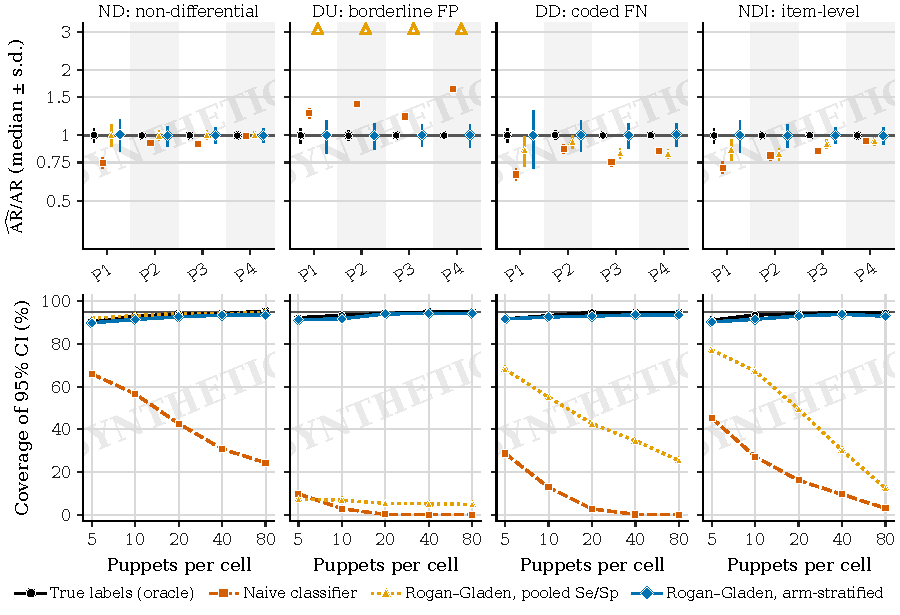
\includegraphics[width=0.94\textwidth]{figures/fig-sim-ar.pdf}
\caption{Synthetic data, E1: estimation of $\mathrm{AR}$ relative to the reverse-chronological reference ($R=1{,}000$ audits per configuration). Top: estimate divided by the true $\mathrm{AR}$, median $\pm$ one Monte Carlo s.d., with $20$ puppets per persona--arm cell; open triangles on the upper edge mark medians beyond the axis (pooled correction under DU, medians $3.4$ to $31$). Bottom: coverage of nominal $95\%$ intervals, averaged over personas, against puppets per cell. ND: non-differential; DU: borderline false positives; DD: coded false negatives; NDI: rates of ND, deterministic per item.}\label{fig:sim-ar}
\end{figure}

\begin{table}[tb]
\centering
\caption{Synthetic data, E1: amplification ratio relative to the reverse-chronological reference, with $20$ puppets per persona--arm cell ($R=1{,}000$; validation of $500$ impressions per arm). Truth: $\mathrm{AR}$ of the pools; it differs between regimes because the avoid-on-flag rule uses the classifier. AR: median estimate. Bias: median relative bias (\%). Cov.: coverage of the nominal $95\%$ interval (\%; MCSE at most $1.6$). RG: Rogan--Gladen correction, error rates pooled over arms or stratified by arm. For the general persona under DU the pooled correction is defined in only $421$ of $1{,}000$ audits, because the corrected reference exposure is otherwise not positive; its median is over those, and the others count as misses.}\label{tab:sim-main}
\footnotesize
\setlength{\tabcolsep}{2.8pt}
\simfit{% Generated by code/make_figures.py from results/sim_results.json -- do not edit by hand.
% E1, reference = chron, 20 puppets per persona-arm cell, validation n = 500 impressions per cell (5 score bands), R = 1000 audits per configuration.
% Truth: pool AR of the regime (regimes differ slightly because the avoid-on-flag choice rule uses the
% classifier). AR: median estimate; Bias: median relative bias (%); Cov.: coverage of the nominal 95%
% interval for AR (%).
\begin{tabular}{@{}llrrrrrrrrrrrr@{}}
\toprule
 & & \multicolumn{3}{c}{P1} & \multicolumn{3}{c}{P2} & \multicolumn{3}{c}{P3} & \multicolumn{3}{c}{P4} \\
\cmidrule(lr){3-5} \cmidrule(lr){6-8} \cmidrule(lr){9-11} \cmidrule(lr){12-14}
Classifier error & Estimator & AR & Bias & Cov. & AR & Bias & Cov. & AR & Bias & Cov. & AR & Bias & Cov. \\
\midrule
Non-differential & Truth & \multicolumn{3}{c}{1.79} & \multicolumn{3}{c}{1.33} & \multicolumn{3}{c}{1.67} & \multicolumn{3}{c}{1.04} \\
 & True & 1.80 & $+$0.2 & 94 & 1.33 & $-$0.2 & 94 & 1.67 & $+$0.0 & 95 & 1.04 & $-$0.2 & 93 \\
 & Naive & 1.34 & $-$25.3 & 0 & 1.23 & $-$7.7 & 50 & 1.52 & $-$8.9 & 27 & 1.04 & $-$0.4 & 94 \\
 & RG pooled & 1.80 & $+$0.4 & 96 & 1.33 & $+$0.0 & 94 & 1.67 & $+$0.2 & 94 & 1.05 & $+$0.3 & 93 \\
 & RG stratified & 1.81 & $+$0.9 & 92 & 1.33 & $-$0.3 & 92 & 1.67 & $+$0.2 & 93 & 1.04 & $-$0.1 & 94 \\
\addlinespace
Differential: borderline FP & Truth & \multicolumn{3}{c}{1.62} & \multicolumn{3}{c}{1.15} & \multicolumn{3}{c}{1.38} & \multicolumn{3}{c}{0.89} \\
 & True & 1.62 & $-$0.0 & 95 & 1.15 & $-$0.3 & 94 & 1.38 & $-$0.1 & 94 & 0.88 & $-$0.1 & 94 \\
 & Naive & 2.05 & $+$26.8 & 0 & 1.61 & $+$39.7 & 0 & 1.69 & $+$22.2 & 0 & 1.45 & $+$63.8 & 0 \\
 & RG pooled & 31.35 & $>{+}10^3$ & 21 & 4.39 & $+$281.6 & 0 & 4.72 & $+$241.8 & 0 & 3.39 & $+$282.8 & 0 \\
 & RG stratified & 1.62 & $+$0.3 & 93 & 1.15 & $-$0.4 & 94 & 1.38 & $+$0.3 & 95 & 0.89 & $+$0.4 & 95 \\
\addlinespace
Differential: coded FN & Truth & \multicolumn{3}{c}{1.82} & \multicolumn{3}{c}{1.36} & \multicolumn{3}{c}{1.78} & \multicolumn{3}{c}{1.07} \\
 & True & 1.82 & $+$0.1 & 95 & 1.36 & $+$0.3 & 94 & 1.78 & $-$0.1 & 94 & 1.07 & $+$0.2 & 95 \\
 & Naive & 1.20 & $-$34.0 & 0 & 1.17 & $-$13.7 & 10 & 1.34 & $-$24.7 & 0 & 0.90 & $-$15.5 & 1 \\
 & RG pooled & 1.55 & $-$14.5 & 80 & 1.27 & $-$6.5 & 83 & 1.47 & $-$17.3 & 6 & 0.88 & $-$17.9 & 2 \\
 & RG stratified & 1.82 & $-$0.1 & 91 & 1.36 & $+$0.4 & 93 & 1.78 & $+$0.2 & 93 & 1.08 & $+$1.0 & 95 \\
\addlinespace
Non-diff. by type, item-level & Truth & \multicolumn{3}{c}{1.82} & \multicolumn{3}{c}{1.30} & \multicolumn{3}{c}{1.69} & \multicolumn{3}{c}{1.03} \\
 & True & 1.82 & $-$0.2 & 94 & 1.30 & $-$0.0 & 95 & 1.69 & $+$0.1 & 94 & 1.03 & $-$0.1 & 94 \\
 & Naive & 1.29 & $-$29.0 & 0 & 1.05 & $-$19.3 & 1 & 1.43 & $-$15.1 & 2 & 0.97 & $-$5.5 & 61 \\
 & RG pooled & 1.57 & $-$13.9 & 70 & 1.07 & $-$17.8 & 12 & 1.54 & $-$8.8 & 49 & 0.97 & $-$6.0 & 67 \\
 & RG stratified & 1.83 & $+$0.4 & 93 & 1.30 & $-$0.3 & 92 & 1.69 & $-$0.0 & 94 & 1.02 & $-$0.4 & 93 \\
\bottomrule
\end{tabular}
}
\end{table}

\paragraph{The reference is part of the estimand} Under ND, $\mathrm{AR}$ is $1.79$, $1.33$, $1.67$ and $1.04$ for the general, Jewish-interest, Middle East and conspiracy-adjacent personas relative to the reverse-chronological feed. It is $2.64$, $1.76$, $2.17$ and $1.29$ relative to the random feed, and $2.76$, $2.05$, $1.17$ and $1.16$ relative to the popularity-only feed, so the ranking of personas changes with the reference (\cref{sec:est-reference}). With true labels, intervals cover in $93.2$--$95.3\%$ of audits with $20$ puppets per cell and in $89.8$--$93.1\%$ with five.

\paragraph{Non-differential error} The naive ratio is attenuated toward one by $25.3\%$, $7.7\%$, $8.9\%$ and $0.4\%$, as \cref{thm:misclass}(a) predicts. The bias does not shrink with more puppets, so coverage falls as the audit grows (general persona: $25.5\%$ with five puppets, $0.0\%$ with $20$). Both corrections have median biases below $1\%$ and coverage of $91.8$--$95.6\%$.

\paragraph{Differential error} For the general persona the algorithm shows more borderline content than the reverse-chronological feed ($11.2\%$ against $3.0\%$ of impressions) and a larger coded share of antisemitic content ($63\%$ against $48\%$). Its specificity is therefore lower under DU and its sensitivity under DD, although no type is classified differently by arm. Under DU the naive ratio is biased upward by $22$--$64\%$, and for the conspiracy-adjacent persona it turns a true $0.89$ into $1.45$. The pooled correction is worse. It subtracts a false-positive rate that is too large for the reference arm, which drives the corrected reference exposure toward zero. For the general persona that exposure was not positive in $579$ of $1{,}000$ audits, and elsewhere the median ratio was $31.3$ against a truth of $1.62$. Under DD the naive ratio is biased by $-14$ to $-34\%$, and for the conspiracy-adjacent persona the naive ($0.90$) and pooled ($0.88$) ratios put a true $1.07$ below one, as in scenario A of \cref{tab:mc-signflip}. The coverage of the pooled correction falls as the audit grows, to $0\%$ for two personas with $80$ puppets. Under NDI each item is always classified in the same way, so an arm's sensitivity depends on which antisemitic items it shows ($0.69$ against $0.79$ for the Jewish-interest persona). Error that is non-differential type by type is then differential by arm, and the naive and pooled ratios are biased by up to $-29.0\%$ and $-17.8\%$. In all three regimes, correction by arm has median biases within $1\%$ and coverage of $90.7$--$95.2\%$.

\paragraph{The price of stratifying} With five puppets per cell, the stratified correction's standard errors are $82$--$94\%$ of the Monte Carlo s.d., and its coverage $88.1$--$94.8\%$. Its mean bias reaches $5.6\%$ because the ratio is skewed, but its median bias stays within $2.5\%$. Validation by arm, as in the protocol (\cref{sec:protocol}), is the safe default; the pooled correction is not.

\subsection{Variance estimators and closed forms (E1b)}\label{sec:sim-checks}

E1b draws $R=2{,}000$ audits from separate pools that record every session. Error rates are known, or estimated externally from $n_1=300$ coded positives and $n_0=1{,}500$ coded negatives (\cref{tab:sim-checks}, \cref{app:sim-further}). As simulated, sessions of a puppet are nearly uncorrelated (design effects $0.96$--$1.23$) and both variance estimators cover. When accounts sit in different experiment buckets, a persistent random shift in the algorithm's weight on bait, the algorithmic arm's design effect rises to $2.75$--$5.65$. Session-level intervals for $\mathrm{AA}$ then cover in only $62.9$--$82.5\%$ of audits, against $93.0$--$93.2\%$ for cluster-robust ones, as \cref{thm:identify}(c) predicts. The form $\mathrm{AR}\,\kappa_a/\kappa_r$ of \eqref{eq:mc-diff} reproduces every naive ratio, and under DD the limit $\mathrm{AR}^{\mathrm{pool}}$ matches the median pooled correction to within $0.006$ (for the conspiracy-adjacent persona both are $0.861$, below one, although the truth is $1.053$). The delta-method s.d.\ of $\log\widehat{\mathrm{AR}}$ understates when $\kappa_{\Sp}=v_{\Sp}^{1/2}/(J\mu_r)$ is large, as \cref{sec:meas-misclass} warns. With $\kappa_{\Sp}\le0.102$, its median over audits is within $-5.3$ to $+3.9\%$ of the Monte Carlo s.d. For the general persona, whose reference exposure is lowest ($\kappa_{\Sp}=0.246$), it understates by $15$--$23\%$, and by up to $33\%$ under DD ($\kappa_{\Sp}=0.312$). Reporting $\kappa_{\Sp}$ and a bootstrap is therefore warranted.

\subsection{Interference (E2)}\label{sec:sim-interference}

Each audit has $15$ protocol puppets per persona and arm (algorithmic, reverse-chronological, popularity-only) and $8$ untrained sentinels, whose openings feed global popularity. The background volume is set so that the puppets generate a share of $0.02$ to $0.3$ of all openings. The load $\bar\ell$ of \cref{sec:id-interference}, the puppets' share of the engagement with the items they open, is then $0.023$ to $0.331$. Each of $R=24$ replications is run at every share with common random numbers, and the bias is the paired difference from the audit without interference. Puppets draw their seeds from the $40$ items closest to their persona. The remedies are low co-viewing (seeds from $200$ items) and staggered waves (five waves, five days apart). Biases are in units of $10^{-3}$ (\cref{fig:sim-interference}; \cref{tab:sim-designs} in \cref{app:sim-further} summarises E2--E5).

\begin{figure}[tb]
\centering
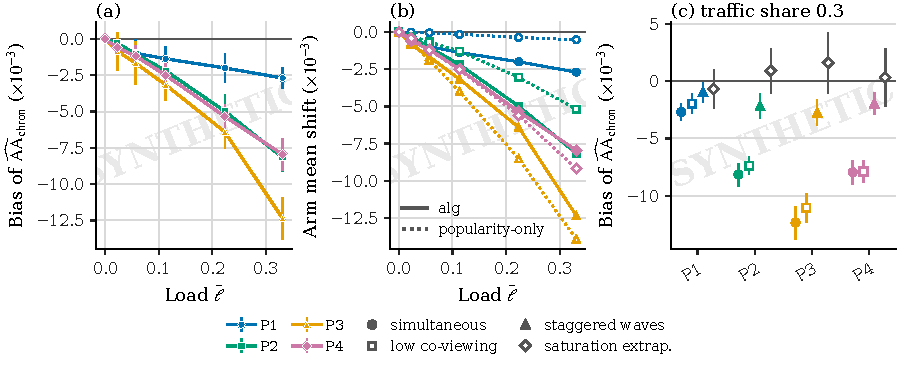
\includegraphics[width=0.94\textwidth]{figures/fig-sim-interference.pdf}
\caption{Synthetic data, E2: interference through shared popularity ($R=24$ paired replications; bars $\pm2$ SE). (a) Bias of the additive amplification relative to the reverse-chronological feed against the load $\bar\ell$, simultaneous design. (b) Shift in mean exposure of the algorithmic arm (solid) and the popularity-only arm (dotted); the reverse-chronological arm does not move. (c) Bias at traffic share $0.3$: simultaneous (load $0.33$), low co-viewing ($0.33$), staggered waves ($0.12$), and randomised-saturation extrapolation from shares $0.1$ and $0.3$.}\label{fig:sim-interference}
\end{figure}

\paragraph{Bias} The bias of $\widehat{\mathrm{AA}}_{\mathrm{chron}}$ is negative for every persona and grows with the load. At share $0.3$ it is $-19$, $-45$, $-23$ and $-247\%$ of the no-audit value, so for the conspiracy-adjacent persona interference reverses the sign of the estimate. Even at share $0.02$ it is $-1.5$ to $-3.5\%$ for three personas and $-19\%$ for the fourth. At share $0.3$, Wald intervals cover in only $25.0$--$70.8\%$ of replications. Exposure under the algorithm and the popularity-only feed falls monotonically with the load, while the reverse-chronological feed, which does not learn, does not move. Avoid-on-flag puppets rarely open antisemitic items, so the popularity they add goes to other items: case (i) of \cref{prop:interference}(b), here over whole sessions. Because the popularity-only feed also learns, the shifts partly cancel. For three personas $\xi_\Delta$ is $0.008$--$0.009$ against that feed and $0.025$--$0.037$ against the reverse-chronological feed.

\paragraph{Remedies} Low co-viewing barely helps, presumably because the seed pool governs only $30$ of a puppet's up to $230$ openings and the first item of each session. Staggering lowers the load to $0.118$ and the bias by $64$--$78\%$. Extrapolating to zero load from shares $0.1$ and $0.3$ (\cref{prop:interference}(c)) leaves biases within $1.2$ SE of zero. It costs $2.3$--$2.8$ times the variance of one audit at share $0.1$, and $4.4$--$5.9$ times for closer loads. The sensitivity interval of \cref{prop:interference}(d), with $\xi_\Delta$ at its simulated value, restores coverage to $95.8$--$100\%$. The breakdown value $\xi^\ast$ is well above the simulated slope only for the Middle East persona ($0.101$ against $0.037$). Sentinel exposure falls by $0.0063$ per unit of load, against $0.0075$--$0.0355$ for the trained algorithmic arms. Sentinels are therefore evidence about $\xi$, not a bound on it.

\subsection{Supply, demand and the fixed-demand audit (E3)}\label{sec:sim-decomp}

The population has $3{,}000$ synthetic users with naturalistic choice and new accounts. Their initial demand $F_0$ is drawn from the four personas (shares $0.6$, $0.1$, $0.15$, $0.15$), with individual noise. Two copies are formed for $H\in\{3,10,20,40\}$ sessions, one under the algorithm and one under the reverse-chronological feed, while demand evolves. Each copy is then evaluated under both policies with demand held fixed, which gives the four cells $\bar\mu(a;b)$ of \cref{thm:decomp} for the same users. The fixed-demand audit holds each user's initial demand fixed in a new account, which is the audit of \cref{prop:audit-scope} at $Q=F_0$.

\begin{figure}[tb]
\centering
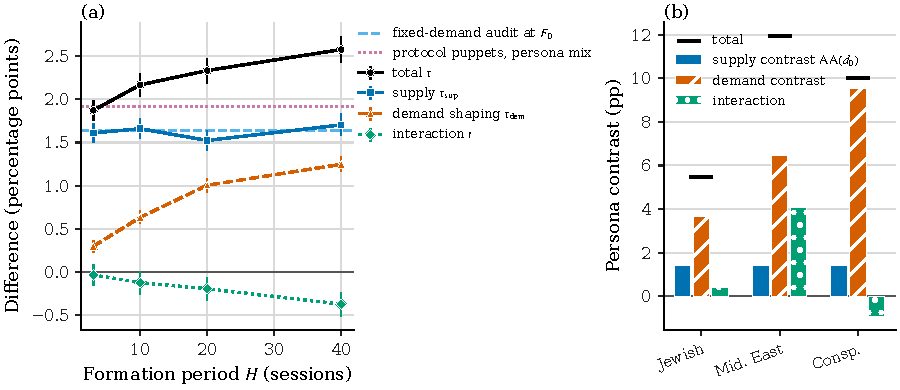
\includegraphics[width=0.94\textwidth]{figures/fig-sim-decomp.pdf}
\caption{Synthetic data, E3: the decomposition of \cref{thm:decomp}. (a) Components for $3{,}000$ synthetic users whose demand evolves, against the length $H$ of the formation period (reference: reverse-chronological; bars $\pm2$ SE over users). Lines: the fixed-demand audit at the initial demand $F_0$, and protocol puppets with the persona mix of the population. (b) Persona-contrast decomposition relative to the general persona $d_0$ (protocol puppets, regime ND); black marks: total $\mu_{\mathrm{alg}}(d)-\mu_{\mathrm{ref}}(d_0)$.}\label{fig:sim-decomp}
\end{figure}

After $40$ formation sessions, the total effect $\tau=2.58$ percentage points (SE $0.08$) splits into supply $\tau_{\mathrm{sup}}=1.70$, demand shaping $\tau_{\mathrm{dem}}=1.25$ and an interaction $\iota=-0.37$ (SE $0.07$). The Shapley shares are $1.52$ and $1.06$, and $\mathrm{TR}=1.45=1.24\times1.17$. As formation lengthens, supply stays between $1.52$ and $1.70$, while demand shaping grows from $0.30$ and the interaction falls from $-0.04$ (\cref{fig:sim-decomp}(a)). The algorithm adds less to demand that it has formed: after $40$ sessions its users draw $7.2\%$ of their pool from borderline and antisemitic sources, against $3.6\%$ under the reference, and the reverse-chronological feed shows those sources too. \Cref{asm:demand} holds closely: no cell differs from fixed-demand accounts with the same demand by more than $0.11$ points (SE $0.05$). The fixed-demand audit gives $\mathrm{AA}=1.64$ points, close to the supply effect. It falls short of the total by $0.23$ points at $H=3$ and by $0.94$ (SE $0.07$) at $H=40$, as \cref{prop:audit-scope} says it must. In the persona contrasts (\cref{fig:sim-decomp}(b)), demand contrasts dominate, but they compare scripts that we chose, not demand formed by the algorithm. The rates at which taste, appetite and follows change are invented. The sizes of $\tau_{\mathrm{dem}}$ and $\iota$, and the sign of $\iota$, belong to these dynamics. E3 shows what a fixed-demand audit targets, not how real demand evolves.

\subsection{Markov predictions and sensitivity (E4)}\label{sec:sim-markov}

For each persona and policy, $250$ naturalistic accounts with fixed demand, which always open an item, run three burn-in sessions. A chain over the states $N$, $B$ and $A$ of the opened items is then estimated from $10$ sessions of $20$ steps (\cref{prop:markov-mle}). It is compared with the same sessions ($e_{20}$), with one further session of $200$ steps ($e_{200}$), and, for $\varpi(\mathcal A)$, with that session's second half. Exposure here counts consumed items.

\begin{figure}[tb]
\centering
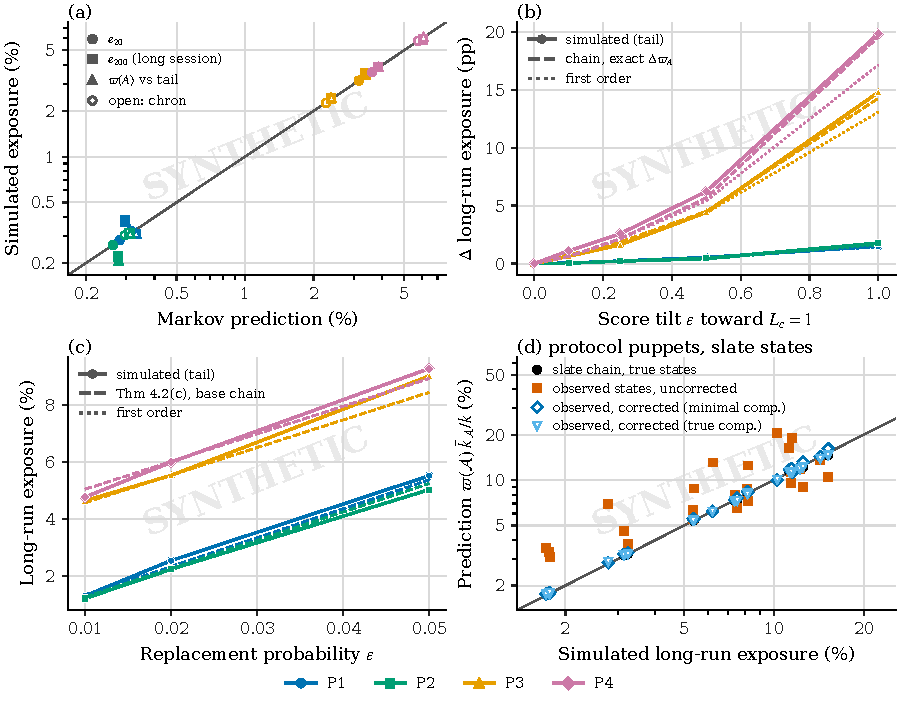
\includegraphics[width=0.94\textwidth]{figures/fig-sim-markov.pdf}
\caption{Synthetic data, E4: Markov chains of consumed items ($250$ accounts per persona and policy). (a) Predictions against simulation for $e_{20}$, $e_{200}$, and $\varpi(\mathcal A)$ against the second half of a $200$-item session; open markers: reverse-chronological. (b) Score tilt $\varepsilon$ toward items with $L_c=1$: simulated change in long-run exposure, the exact change between the estimated chains (\cref{thm:perturb}(a)), and its first-order term. (c) Replacement of the next item by an antisemitic one with probability $\varepsilon$: simulation, the closed form of \cref{thm:perturb}(c) from the base chain alone (dashed), and its first-order term $\varpi(\mathcal A)(1+\varepsilon\,\E_\varpi\tau_A)$ (dotted).}\label{fig:sim-markov}
\end{figure}

The chain reproduces $e_{20}$ within $0.0002$ in all eight cells, which is an in-sample check. Out of sample, $e_{200}$ is predicted within $7\%$ in six cells. It errs by $-22\%$ and $+26\%$ in the algorithmic arms of the general and Jewish-interest personas, where exposure is rarest (about $0.3\%$) and $\varpi(\mathcal A)$ misses the second-half share by up to $34\%$. At the audited horizon, session averages should remain primary (\cref{sec:markov-estimation}). The chains mix fast: Kemeny's constant is $1.98$--$2.17$ and $\kappa_{\mathcal A}$ is $0.50$--$0.52$ in every cell. This world therefore lacks the sticky regions in which \cref{thm:perturb} predicts the largest magnifications. When the algorithm's score of antisemitic items is tilted, the exact identity of \cref{thm:perturb}(a), applied to the estimated chains, tracks the simulated change (at $\varepsilon=1$, $14.26$ against $14.77$ percentage points for the Middle East persona). The bound of part (b) holds but is loose. It exceeds the exact change by factors of $1.3$--$3.3$ for the Middle East and conspiracy-adjacent personas and $3.2$--$120$ for the other two, because $\|P_1-P_0\|_\infty$ includes the rarely visited, noisily estimated row of $A$. When the next item is replaced by an antisemitic one with probability $\varepsilon\le0.05$, the closed form of \cref{thm:perturb}(c), computed from the base chain alone, predicts long-run exposure within $9\%$. Its multiplier shows. For the general persona, with $\E_\varpi\tau_A=345$ items, replacing $1\%$ of items raises long-run exposure from $0.31\%$ to $1.30\%$. For the Middle East persona, which reaches antisemitic items quickly anyway, it rises from $3.56\%$ to $4.64\%$.

\subsection{The sequential audit (E5)}\label{sec:sim-sequential}

Pairs of one algorithmic and one reverse-chronological puppet are resampled from the E1 pools (regimes ND and DD) and arrive in waves of five. Each puppet codes $m=10$ flagged positions, giving $Y_u=\bar Q_u\widehat P_u$, and \cref{alg:sequential} runs with the mixture tuned to $t^\ast=40$ pairs. There are $R=2{,}000$ audits of up to $400$ pairs ($80$ waves) per configuration. In the null case both arms come from the reference pool. The sensitivity ratio is $\lambda_S=1.00$ under ND, and $0.86$, $0.93$, $0.83$ and $0.82$ under DD. Stopping is evaluated at the settings for which the protocol was first written: $\alpha=0.0125$ per persona, $\delta=1.25$, $b=1$ burn-in wave, and $W_{\max}=8$ waves of five pairs. \Cref{sec:protocol} explains why the registered design is larger.

\begin{figure}[tb]
\centering
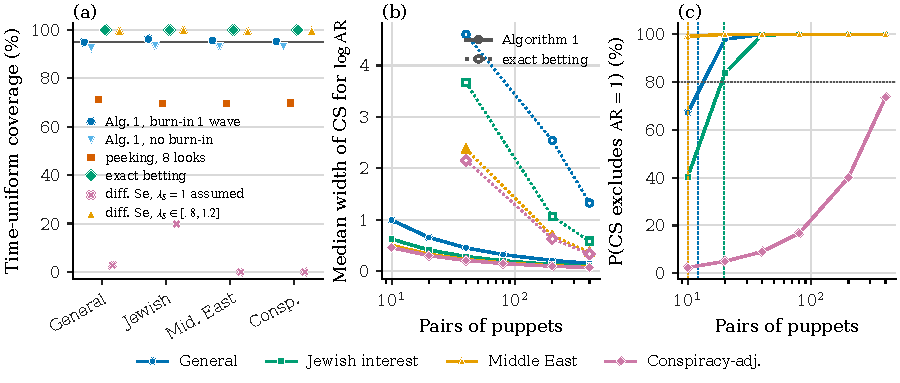
\includegraphics[width=0.94\textwidth]{figures/fig-sim-sequential.pdf}
\caption{Synthetic data, E5: \cref{alg:sequential} against the reverse-chronological reference, waves of five pairs ($R=2{,}000$; exact betting $R=200$). (a) Time-uniform coverage at $\alpha=0.05$ over $80$ waves, with and without one burn-in wave; a fixed-sample interval recomputed after each of the first eight waves (peeking); exact betting; and, under DD, $\lambda_S=1$ assumed or the range $[0.8,1.2]$. (b) Median width for $\log\mathrm{AR}$: \cref{alg:sequential} (solid), exact betting (dotted). (c) Probability of excluding $\mathrm{AR}=1$; dashed verticals: the horizon $n_{\mathrm{seq}}$ of \cref{prop:power}(d), at least two waves (beyond the axis for the conspiracy-adjacent persona).}\label{fig:sim-sequential}
\end{figure}

\paragraph{Coverage and peeking} With one burn-in wave, time-uniform coverage over $80$ waves at $\alpha=0.05$ is $95.0$--$96.2\%$, and $95.0$--$96.3\%$ under the null. Without it, coverage is $92.6$--$93.5\%$ and $92.0$--$94.0\%$: the first wave, with five pairs and a skewed $Y_u$, is where the normal approximation fails (\cref{sec:meas-sequential}). At $\alpha=0.0125$ (nominal $98.75\%$), coverage is $98.0$--$98.8\%$ with the burn-in and $96.0$--$97.0\%$ without, so the relative excess of the miss rate is largest at the per-persona level. A fixed-sample interval recomputed after each of the first eight waves covers at every look in only $69.5$--$71.2\%$ of audits. Under the null it rejects $\mathrm{AR}=1$ at some look in $29.2$--$33.0\%$ of audits, against $2.1$--$3.4\%$ for \cref{alg:sequential}. Most of the excess over the $17.6\%$ of \cref{sec:meas-sequential} comes from the first look.

\paragraph{Conclusions on the original budget} Under ND, the audit contradicts the true $\mathrm{AR}$ in at most $0.05\%$ of audits. It concludes material amplification for the general persona ($\mathrm{AR}=1.79$) in $85.8\%$ of audits, after $5.1$ waves on average, and for the Middle East persona ($1.67$) in $99.9\%$, after $2.8$. It concludes no material difference for the conspiracy-adjacent persona ($1.04$) in $91.2\%$. For the Jewish-interest persona, whose ratio of $1.33$ lies just above $\delta=1.25$, it detects a difference by wave $8$ in $98.7\%$ of audits, but materiality stays undetermined in $93.8\%$ within the eight-wave budget, and in $64.1\%$ even after $40$ waves. Under the null, wrong conclusions occur in $0.20$--$1.05\%$ of audits with the burn-in, within the per-persona level of $1.25\%$, and in up to $2.95\%$ without it.

\paragraph{Power} The closed form $A_Y$ of \cref{prop:power}(d) overstates the simulated variance by $5$--$23\%$, which is conservative. The simulated power for detecting $\mathrm{AR}\ne1$ is $0.82$--$0.93$ at $n_{\mathrm{fix}}$ and $0.85$--$1.00$ by $n_{\mathrm{seq}}$ (\cref{tab:sim-designs}). With $\lambda_S\in[0.95,1.05]$, no horizon exists for the conspiracy-adjacent persona, since $|\log\mathrm{AR}|=0.042<\log(1.05/0.95)$. The exact betting sequence covers in all $200$ of its audits but is nearly powerless here: its median width at $40$ pairs is $2.2$--$4.6$, against $0.21$--$0.45$ for \cref{alg:sequential}.

\paragraph{Differential sensitivity} Under DD, assuming $\lambda_S=1$ gives coverage of $2.8$, $19.8$, $0.0$ and $0.0\%$, because the sequence then covers $\lambda_S\mathrm{AR}$, not $\mathrm{AR}$. For the conspiracy-adjacent persona ($\mathrm{AR}=1.07$, $\lambda_S\mathrm{AR}<1$), the audit detects de-amplification within eight waves in $48.5\%$ of audits. The range $[0.8,1.2]$, which contains every $\lambda_S$ of the regime, restores coverage to $99.4$--$100\%$ and removes the wrong conclusions, but takes most of the power with them. By wave $8$ the sequence excludes $\mathrm{AR}=1$ in $49.6$, $5.5$, $92.8$ and $0.0\%$ of audits, against $96.1$, $85.0$, $100$ and $54.8\%$ with $\lambda_S=1$.

\subsection{What the simulation does and does not show}\label{sec:sim-scope}

Where their conditions hold, the results of \cref{sec:estimands,sec:markov,sec:identification,sec:measurement} hold in finite samples: corrections by arm, cluster-robust intervals, the closed forms of \cref{thm:misclass,thm:perturb}, the scope of fixed-demand audits (\cref{prop:audit-scope}), and \cref{alg:sequential} with one burn-in wave at $\alpha=0.05$. The methods also fail where the theory says they will. Error that depends only on content still differs between arms, and then the naive ratio and the pooled correction can lie on the wrong side of one. The pooled correction explodes when the corrected reference exposure nears zero. Interference can reverse the sign of the additive amplification. Assuming $\lambda_S=1$ under differential sensitivity gives $0$--$20\%$ coverage, and a declared range that contains $\lambda_S$ restores it, at the cost of power. Approximations show at these sizes. The miss rate of \cref{alg:sequential} reaches $2.0\%$ against $1.25\%$ at the per-persona level, the delta-method s.d.\ understates when $\kappa_{\Sp}$ is large, Markov extrapolation to long sessions errs by up to $26\%$, and the bound of \cref{thm:perturb}(b) is loose. On the original eight-wave budget, materiality stays undetermined for the persona whose ratio lies near the margin.

The simulation does not show how any real recommender behaves. The world, the classifier, the personas and the demand dynamics are invented, and the ratios from $0.89$ to $2.76$, the interference biases and the decomposition shares follow from our parameters. Parts of the protocol were not simulated. E5 evaluates \cref{alg:sequential} on the confirmed-flagged statistic, with pairs resampled independently from fixed pools: no drift, interference, attrition or coder error. It uses ten sessions and slates of four, and it evaluates neither the sequence on double-sampled exposures nor the sample sizes of the registered design (\cref{sec:protocol}). E4 models the opened items of naturalistic accounts, not the slate states of the protocol, and its fast-mixing chains do not test the sticky regime. E2 has one interference channel, $24$ replications, and no load below $0.023$. E3 rests on dynamics of demand for which we have no evidence. And because puppets and users are served by the same rules by construction, the transport condition (\cref{asm:id-transport}), which a real audit can least check, is never at risk.
